\chapter{Performance of Gaussian smoothing}
\label{APP::SMOOTHING}

The performance of the Gaussian smoothing, $g(\vec{r})$, and the
``Trashcan'' smoothing, $t(\vec{r})$ from \citet{REF::LESSARD::2001APP}
can be evaluated using a simple Monte Carlo simulation. The 
smoothing functions are given by,
\begin{eqnarray*}
g(\vec{r}) & = & \exp(-r^2/2\,r_0^2) \\
t(\vec{r}) & = & \left\{1\,(r<r_0) \atop 0\,(r>r_0)\right.
\end{eqnarray*}

A simple sky-map can be produced given a background rate ($r_b$), a
\Gray signal rate ($r_s$), and a value for the intrinsic angular 
resolution of the two dimensional reconstruction method before
smoothing ($\sigma_\mathrm{2D}$). Appendix~\ref{APP::ELLIPT} indicates
that $\sigma_\mathrm{2D}=0.2^\circ$ is reasonable. The background and
signal in each bin of the sky-map are given by a Poisson distributed
random deviate with appropriate mean, denoted $B(\mu_B)$ and
$S(\mu_S)$ for the case of mean background $\mu_B$ and mean signal
$\mu_S$. The background is distributed uniformly over both the
\On\ and \Off\ maps, while the signal appears only in
the \On\ source map and is smeared over a number of bins by the
point-spread function. A simple Monte Carlo simulation of a typical
sky-map is as follows,
\begin{eqnarray*}
OFF(\vec{r'}) & = & B(r_b) \\
ON(\vec{r'}) & = & B(r_b) + S\left(\frac{r_s}{2\pi\sigma_\mathrm{2D}^2}e^{-r^2/2\sigma_\mathrm{2D}^2}\right)
\end{eqnarray*}

To evaluate the performance of the smoothing algorithms, the sky-map
is be smoothed with both smoothing functions ($g(\vec{r})$ and
$t(\vec{r})$), and the significance calculated from
equations~\ref{EQN::ANALYSIS::SMOOTHEXCESS} and
\ref{EQN::ANALYSIS::SMOOTHDELTAEXCESS}. Figure~\ref{FIG::APPSMOOTHING::SIGMA}
shows the average, maximum significance calculated over a large number
of smoothed sky-maps, as a function of the smoothing radius, $r_0$.
Values of $r_b=30\,\mathrm{count/bin}$ and $r_s=1000\,\mathrm{counts}$
were used, which are reasonable for a bright source.

\begin{figure}[ht]
\centerline{\resizebox*{\textwidth}{!}{\rotatebox{270}{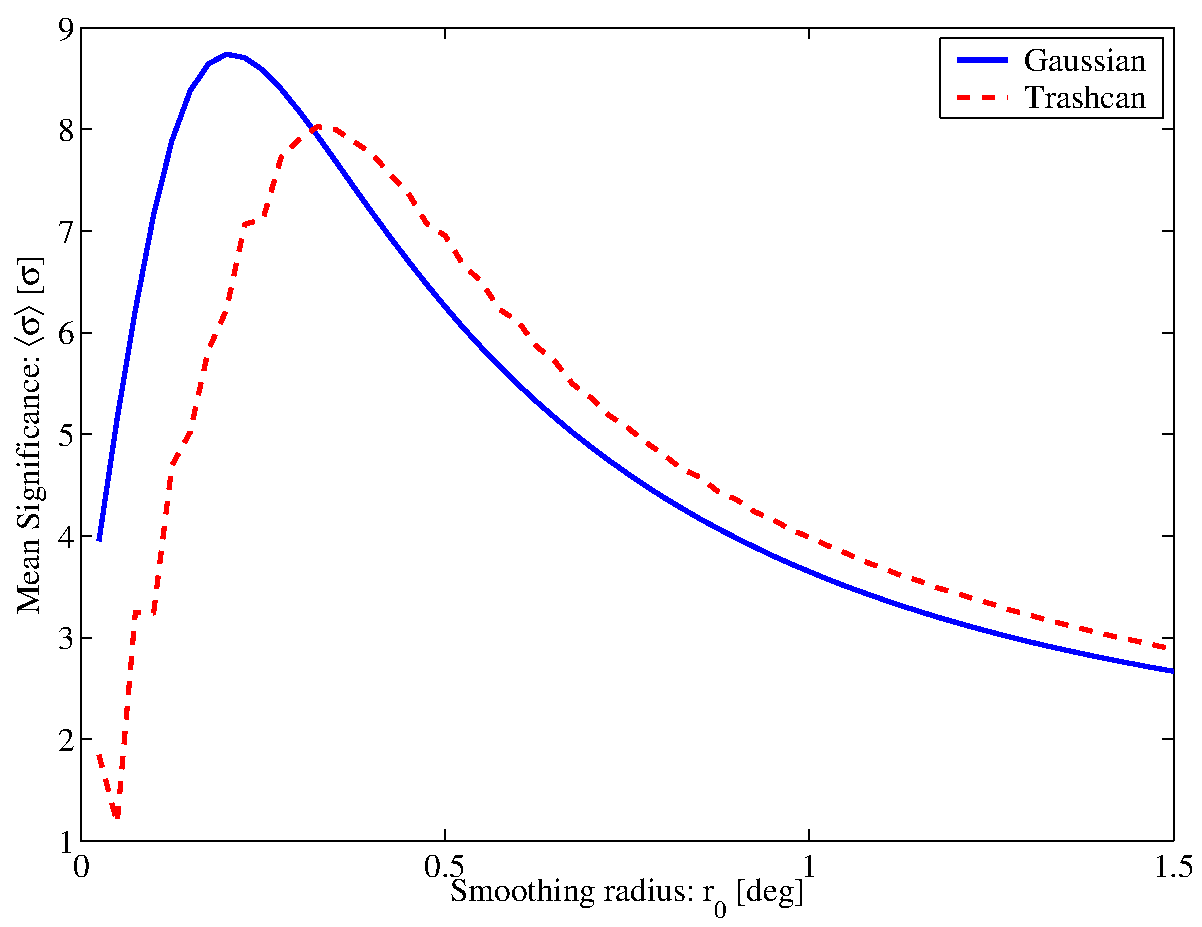
\includegraphics[draft=false]{plots/app-smoothing/smoothing.pdf}}}}
\caption{\label{FIG::APPSMOOTHING::SIGMA} Mean significance after smoothing
with Gaussian and Trashcan functions with various smoothing radii.} 
\end{figure}

On average, the Gaussian smoothing function performs slightly better,
with $\langle\sigma\rangle$=8.75$\sigma$ for $r_0=0.2^\circ$, while
the Trashcan function has maximum mean significance of
$\langle\sigma\rangle$=8.0$\sigma$ for $r_0=0.325^\circ$.

Finally, by removing the \Gray source from the Monte Carlo
simulations, distributions of the maximum significance in the absence
of a source, can be calculated for various regions of the sky-map. The
results of this analysis, for regions of $R<0.35^\circ,\,
<0.55^\circ,\, <1.10^\circ$ are presented in
figure~\ref{FIG::ANALYSIS::2DSIGMADISTRIBUTIONS}, along with
experimental distributions and a theoretical curve based on the
assumption that the counts are distributed as Gaussian.
